
%\documentclass[a4,technote,12pt,twoside]{ieeetran}
%\documentclass[a4,12pt,twoside]{ieeetran}
\documentclass[twocolumn]{IEEEtran}

%\usepackage[dvips]{epsfig} 
%\usepackage{subfigur} 
\usepackage{alltt,graphicx}%,
\usepackage[letterpaper,pdftitle={ISIC Paper},pdfauthor={Zhen Song}, pdfkeywords={ Hough transform; line fitting; corner fitting; arc/circle fitting; ellipse fitting; algebraic fitting; Omni-directional vehicle (ODV)} ]{hyperref}
\usepackage[centertags]{amsmath}
%\usepackage{amsfonts}
%\usepackage{amssymb}
%\usepackage{amsthm}
%\usepackage{newlfont}
\bibliographystyle{ieeebib}
\renewcommand{\baselinestretch}{0.90}
\thispagestyle{empty}
\pagestyle{empty}

\begin{document}
  

%\title{Title of Paper to be Presented at CCA\thinspace'01 or ISIC\thinspace'01}
%
%\author{\vskip 1em
%Author(s)\\
%\vskip 1em
%{\small Affiliation\\
%Department/Institute\\
%Street, City, State, Postal Code, Country\\
%{\tt E-mail}\\
%\vskip -0.5em
%{\tt URL}}}


\title{%{\vspace*{-1cm} \hspace*{12.5cm} \Large \bf IEEE ISIC'02}
%\\ \Large \bf  
\LARGE \bf Some Sensing and Perception Techniques for an Omnidirectional Ground Vehicle
with a Laser Scanner
\thanks{%Jan. 2002.  {\em For submission to IEEE International Symposium on Intelligent Control (ISIC'02)},  Oct. 2002, Vancouver, Canada, as an invited session paper.   Invited Session   organized by Dr  Jason Gu.
   The authors are with the Center for Self-Organizing and Intelligent Systems (CSOIS), Dept. of Electrical and Computer Engineering,  4160 Old Main Hill, Utah State University, Logan, UT 84322-4160, USA. 
    This work is supported in part by U.S. Army Automotive and Armaments Command (TACOM)
 Intelligent Mobility Program (agreement no. DAAE07-95-3-0023). Corresponding author: Dr YangQuan Chen. E-mail:  \texttt{yqchen@ieee.org}; Tel. 01-435-7970148; Fax: 01-435-7972003. URL: \texttt{http://www.crosswinds.net/\char126 yqchen}. } 
}


\author{\vskip 1em
Zhen Song,   YangQuan Chen,  Lili Ma and   You Chung Chung \vskip 1em }
 


\maketitle

\begin{abstract}                          % Not more than 200 words.
This paper presents some techniques for sensing and perception for an
omnidirectional ground autonomous vehicle equipped with a laser scanner. In an
assumed structured environment, the sensor data processing methods for both 1D
and 2D laser scanners, are discussed. Raw data are segmented to lines, circles,
ellipses, planes and corners by task dependent segmentation algorithms.  Each
subset of data is then fit by known template shapes as listed above.  An arbitrator is used to discriminate the shape for the final object identification.
%\begin{keyword}   % Five to ten keywords,  
\\
{\bf Key Words: } 
 Hough transform;
 line fitting;
 corner fitting;
 arc/circle fitting;
 ellipse fitting;
 algebraic fitting;
 object arbitrator;
 %geometrical fitting;
 Omni-directional vehicle (ODV).
%\end{keyword}                             % keyword list.
\end{abstract}

% sorry, I have to use the following preambles
% apologize for any inconvenience caused!

\newtheorem{remark}{Remark}[section]
%%% defines the QED square and the proof environment
%\def\QED{~\rule[-1pt]{5pt}{5pt}\par\medskip}
%\newenvironment{proof}{{\bf Proof: \ }}{ \hfill \QED}
\def\etal{ {\em et  al. }}
\def\K{ $^\circ{\rm K}$ }
\def\norml{\parallel\!\!}
\def\normr{\!\!\parallel}
\def\eqdef{\stackrel{\triangle}{=}}
\def\rd{\partial}
\def\ba{\begin{array}}
\def\ea{\end{array}}                                    
\def\be{\begin{equation}}
\def\ee{\end{equation}}
\def\bi{\begin{itemize}}
\def\ei{\end{itemize}}
\def\bea{\begin{eqnarray}}
\def\eea{\end{eqnarray}}
\def\btb{\begin{tabular}}
\def\etb{\end{tabular}}
\def\bbm{\begin{bmatrix}}
\def\ebm{\end{bmatrix}}
\def\bpm{\begin{pmatrix}}
\def\epm{\end{pmatrix}}
\def\mb#1{{\mathbf #1}}
\def\ne{ \nonumber \\ \, }
\def\ca{\citeauthor}
\def\bq{\begin{quote} \sf}
\def\eq[#1]{\hfill \textrm{#1} \end{quote}}

\def\d{ {\rm  d} }
\newtheorem{thm}{Theorem}[section]
%\newtheorem{remark}{Remark}[section]

%%%%%%%%%%%%%%%%%%%%%%%%%%%%%%%%%%%%%%%%%%%%%%%%%%%%%%%%%%%%%%%%%%%%%%%%%%%%
\thispagestyle{empty}
\section{Introduction}
\label{sec1}
%%%%%%%%%%%%%%%%%%%%%%%%%%%%%%%%%%%%%%%%%%%%%%%%%%%%%%%%%%%%%%%%%%%%%%%%%%%%   
 

%{\em To be finished by Dr Chen.}

\subsection{Motivation}

For any intelligent mobile robot, the perception of its environment via suitable sensing capacities plays a key role~\cite{Adams99,Nourbakhsh97}. The  environment perception depends largely on the properties of environment itself. Basically, the environment can be assumed to be either static (deterministic) such as office corridor  or dynamic (changing) such as a   parking lot with vehicles in and out dynamically. In terms of deterministicism of the environment, there are two types: deterministic environment and uncertain environment.
With combination, we have four types of environments: static deterministic, dynamic deterministic, static uncertain and dynamic uncertain. For static and dynamic deterministic environments, the sensing and perception task is easier with a help of a map and the known motion patterns of the objects in the environment. For uncertain environment, it seems that no {\em off-the-shelf} solution exists for general sensing and perception tasks for mobile robots \cite{Adams99}. This is because,  sensing and perception  solutions  are usually {\em platform-specific}  for mobile robot with given or existing sensing capability~\cite{Adams99,Nourbakhsh97}. However, there are still some common and possibly low-level solutions applicable for all platforms. This paper attempts to present some commonly used  techniques for sensing and perception for  mobile robot equipped with a 1D or 2D laser scanner in static uncertain environment.
Our test platform is an omni-directional ground autonomous vehicle developed in the CSOIS at Utah State University (USU).



Our approach for static uncertain environment perception is based on the following steps (1) laser scanner raw data collection, (2) segmentation, (3) fitting from the object library (or object templates), (4) object arbitration or decision. 
For step-1, pre-processing is performed to reject some obviously abnormal points or outliers.
In step-2, the range data array from a laser scan is to be segmented to form some subsets of point clouds containing essential information for the object fitting. We assume that a library of objects such as line, corner/rectangle, arc/circle/ellipse etc. are available from the prior knowledge about the static uncertain environment.
Then, in step-3, we fit the through the library since we do not know in advance which object the given point cloud represents. The arbitration or decision on which object in step-4 is done by a rule based comparison of the fitting scores. We believe that this procedure is natural and can be regarded as a common piece of utility in sensing perception using a laser scanner. In each step of the above proposed procedure, there are many technical as well as theoretical challenges. In the present paper, we shall be more focused on step-2 and step-3. 

One of the major contributions of this paper is the collection of some commonly used object fitting algorithms well tested in our experiments with our C++ and Matlab codes publically available 
\footnote{\texttt{http://www.csois.usu.edu/code2share/isic2dlaser.zip}}.


\subsection{The USU ODIS/T4 Platform}

The USU ODIS  robot is   a small, man-portable mobile robotic system that can be used for autonomous or 
 semi-autonomous inspection under vehicles in a parking area \cite{moore_csm}. Customers for such a system include military police (MP) and other law enforcement and security entities. The robot features (a) three ``smart wheels''  in which both the speed and direction of the wheel can be independently controlled, (b) a vehicle electronic capability that includes multiple processors, and (c) a sensor array with a laser, sonar and IR sensors, and a video camera. ODIS employs a novel parameterized command language for intelligent behavior generation. A key feature of the ODIS control system is the use of an object recognition system that fits models to sensor data. These models are then used as input parameters to the motion and behavior control commands.
Figure~\ref{fig:odis1} shows the mechanical layout of the ODIS robot. The robot is 9.8 cm tall and weighs approximately 20 kgs. Key ODIS subsystems include its mechanical, vehicle electronics (vetronics) and sensor systems.  For more detailed description, see ~\cite{odis_spie01},~\cite{odis_icra01}.

\begin{figure}[!htb]
        \center
        \includegraphics[width=0.25\textwidth]{img/odis1}
        \caption{The mechanical and vetronics layout of ODIS}  \label{fig:odis1}
\end{figure} 

%Figure~\ref{odis1blk} shows the behavior control architecture that has been developed. Starting from the "inside out," the control architecture contains two inner motion-control loops. The inner most loop is the wheel-level control, which acts to drive each smart wheel to its desired steering and drive speed set-points. The wheel-level controller uses simple PID control algorithms. Around the inner loop is the path-tracking controller. This loop derives the set points need by the wheel-level control in order to force the vehicle to follow a desired path in space, where a path is defined as an arc in inertial space (with a prescribed velocity along the arc) and an  associated vehicle yaw motion. The path-tracking controller uses a newly-developed spatial tracking control algorithm that is described in more detail in  \cite{odis_icra01}. 


Figure~\ref{fig:1dlaser} shows the 1D laser scan data for a typical set of objects in front of the ODIS equipped with a 1D laser. %add new
Though 1D laser scanner can not change its yaw angle itself, ODIS can. To get 2D information, ODIS rotates with respect to the center of its mass while firing its 1D laser. By this way, the 1D laser system can get 2D point cloud. 
In our project, objects in parking lots can be  decomposed into  combinations of  arcs/circles and lines/rectangles. 

\begin{figure}[!htb]
    \begin{minipage}[t]{0.24\textwidth}
    \center\includegraphics[width=\textwidth]{img/1Dlaser}
    \caption{1D Laser Data (Top: Object Setting.  Bottom: Laser Data)}
        \label{fig:1dlaser}
    \end{minipage}%
    \begin{minipage}[t]{0.24\textwidth}
        \center
        \includegraphics[height=\textwidth, width=\textwidth]{img/2Dlaser}
        \caption{The 2D Laser Scanner Coordinate System}  \label{fig:2dlaser}
    \end{minipage}
\end{figure}

Currently, the cost of a 2D laser scanner is greatly reduced, which enables increasingly many robots be equipped with a 2D laser scanner. The 2D laser scanner is mounted on a servo system that can change the pitch angle. While the 2D laser scanner is shining the laser, the pitch angle can be changed smoothly. Then we can get 3D point cloud. Again, ``{\em off-the-shelf}'' algorithms for object identification or for environment features extraction have not been available although some very platform-specific schemes are proposed or tried, e.g., the research work reported in \cite{Dedieu00Mixed,Hartmart2001ISR,Taylor1996,Vandorpe1996,Cadenat2000,Laurent1997,Borenstein96WhereAmI}. %The "cite" can't be too long for the first time
Figure~\ref{fig:2dlaser} shows the coordinate system of the 2D SICK laser \footnote{\texttt{http://www.sickoptic.com/kommerce\_server/}}, which, for computational  convenience, is different from the body frame coordinate system (BFCS) and inertial coordinate system (ICS). The height of 2D laser above ground, denoted by $h$,  is  constant. From the data of 2D laser scanner, we can get a set of raw data points $(x',y')$ together with  the corresponding pitch angle $\alpha$ from the pitching servo system. To convert the raw data into 3D coordinate system $(x,y,z)$, we have
$   \beta={\rm atan} (y'/x')  $ and $ d = \sqrt{x'^2 + y'^2} $. So, $ (x,y,z)=(d \cos(\beta)\sin(\alpha), d \sin(\beta), h-d \cos(\alpha)\cos(\beta) )$.
In Sec.~\ref{sec3}, we will introduce some object fitting algorithms such as plane fitting (Sec.~\ref{sec3_planefit}), 3D corner detection  and  fitting (Sec.~\ref{sec3_3dcornerfit}), and etc. for 2D laser scanner.


%***************************************************
\nopagebreak
\section{Segmentation}
\label{sec2}


\subsection{Line Detection for Segmentation}
\label{sec21}

Line detection is the first step to segment 1D laser data. After the line detection, we can judge if a point is on the line by checking the distance from the point to the line. In our project, it is reasonable to segment objects in parking lots into circles and lines. So, segmentation is simplified as line detection and circle fit. 

Among many published methods on line detection, some took the frequency-domain approach ~\cite{HuaLineFitting} and others took time-domain approach, e.g., Hough transform ~\cite{HoughSurvey}, or color pattern analysis~\cite{Jan00model}. In our project, the input is the sequential laser range data, instead of an image. In the following discussion, we will focus on Hough transform.

Hough transform (HT) is a popular method for the extraction of geometric primitives \cite{HoughSurvey,Atherton99CHT}. Initially, it is only an approach for line detection. Later, many variants are developed to detect circle~\cite{Atherton99CHT}, ellipse~\cite{guil97lower}, or more complex binary patterns~\cite{guil96new}. A survey on Hough transform can be found in~\cite{HoughSurvey}. 

Generally speaking, HT is robust to sensor noise at the expense of slow computation. The computational cost of the traditional HT is ${\cal O}(n^3)$ where $n$ is the number of data points. Though some efforts were made to speed up the HT algorithm~\cite{matas98progressive}, those fast strategies were developed generally for image data processing applications only. 

However, in our case, a 1D laser data set contains only {\em sparse}  binary information in the region of interest. Furthermore,  only a 1D array is required for laser data instead of a 2D  matrix for the image data. More importantly, the laser data set is  sequential or ordered. Taking these properties of laser data set into consideration, HT can be modified to reduce the computational time. 

\subsection{Sparse Hough Transform for 1D Line Detection}
\label{sec22}

In order to make the best use of the above mentioned features of laser scanner data set, here we propose a sparse Hough transform (SPHT) that fits better to the laser data processing problem. The standard Hough transform (SHT) represents lines crossing a point by 
$$ \rho = x \cos\theta + y \sin\theta, $$
where $\rho$ and $\theta$ are the length of the normal and the angle of the normal with respect to the positive $x$-axis. $x$ and $y$ are the coordinates of a point of interest in the image.   $\rho$ and $\theta$ are quantified as an accumulator matrix. The value of each cell of the matrix represents how many times there is a line, denoted by $(\rho, \theta)$, passing a point in the image. The idea of SHT is to provide an equivalent but faster and less memory-demanding approach. %add new
The inputs and outputs of the SPHT algorithm are {\em exactly} the same as SHT, except that in sparse cases SPHT saves time and memory. Here sparse means both the number of data points and the number of the lines passing these points are small, which is true in our case. Basically, SPHT does not use a 2D array to record the votes. Instead, it uses a 1D  array for the  vote-counting. Since in sparse case, most lines passing one point are not the fitted line, we can compute only those lines that pass at least two points in the image. Transferring all the lines corresponding to one point in the image plane, as SHT does, will take extra computer memory and reduce the speed. 


Based on the above considerations, we present an 
 implementation of SPHT by the following   pseudo-code list:\\
(\texttt{Dat} is the input array; \texttt{Dat(n).x} is the $x$ value of the $n$-th point. 
\texttt{Lines} is the output array that stores $(\rho,\theta)$ of the fitted lines.
\texttt{NumLen} is the number of the fitted lines.)

{\small \noindent
\texttt{NumLen=0}\\
\texttt{for i=1 to n-1}\\
\hspace*{4mm}    \texttt{for j=i+1 to n} \\
\hspace*{8mm}                $\alpha$ = atan($\frac{ Dat(i).y- Dat(j).y}{Dat(i).x - Dat(j).x} $)\\
\hspace*{8mm}                $\rho_0$ =Dat(i).x cos($\alpha$ -$\pi$/2) + Dat(j).y sin($\alpha-\pi/2$)\\
\hspace*{8mm}                $\theta$= $\alpha$-sign($\rho_0$) $\pi/2$ \\
\hspace*{8mm}                $\rho=|\rho_0|$ \\
\hspace*{8mm}                Cell$\theta$=floor($\theta$/$\Delta\theta$)*$\Delta\theta$ \\
\hspace*{8mm}                Cell$\rho$=floor($\rho/\Delta\rho$)*$\Delta\rho$ \\
\hspace*{8mm}                If the line $n$, where $n\in[1,\mbox{\tt NumLen}]$, is close enough to (Cell$\rho$,Cell$\theta$), increase the vote of Lines($n$) by one, otherwise {\tt NumLen=NumLen+1}, and add a line (Cell$\rho$, Cell$\theta$) to Lines with the vote equals to one.  \\
\hspace*{4mm}    \texttt{end for} \\
\texttt{end for}
}
    
Figure~\ref{fig:spht} shows an example of the proposed SPHT. The SPHT transforms or fits  the raw data set to 2 lines. Actually,  the raw data could be interpreted as 2 lines,  or 2 lines plus a small transition arc, or even just one line. The exact segmentation depends on the resolution, or the threshold. For example, with a  precise laser sensor, we know  that the data in Fig.~\ref{fig:spht} cannot be a single line. However, with a low-precision sonar sensor, the target object might be just a single line. With a given sensor in real project, we should choose some reasonable thresholds by referring to the specifications of the sensors. Further discussions on the trade-off between sensor accuracy and the object fit accuracy can be found in~\cite{Goto98Efficient} and ~\cite{Goto00Design}.


\subsection{Analysis on Speed and Memory Size}
\label{sec23}

In general, suppose that the angle resolution is denoted by $\Delta\theta$ and the normal resolution by  $\Delta\rho$. For SHT, $M\times N$ cells are required for the accumulator space, where $ M = \pi/\Delta\theta $ and  $N=\rho_{max}/\Delta\rho.$
In other words, the   memory size is $n\times M\times N$, where $n$ is the size of each cell.
If there are $K$ valid points in the input data, the computation requirement is ${\cal O}(K\times M)$.

For SPHT, if there are only $K$ valid points in the input, clearly, $K\ll M$ and $ K \ll N$. The maximum number of fitted lines will be $ K\times (K-1)/2$. The computation requirement is ${\cal O}(K\times (K-1)/2) $. The actual memory requirement depends on how many lines passing the data points in the input data. Normally, we expect that the number of lines, $L$, for our data is 2 to 4. It is easy to show that $L\leq K(K-1)/2$. 

In~\cite{GieslerLogHough}, another scheme called Log-Hough transformation (LHT) was described. This algorithm is fast, with the complexity of ${\cal O}(n)$, and easy to implement. The authors introduced the concept of logarithmized cosine curve. For an arbitrary set of points, we can store the logarithmized cosine curve of a point of the set in a look-up table, then shift it by other parameters. The following is a comparison between the LHT  and the SPHT:\\
\begin{itemize}
    \item Memory: The exact memory requirement of SPHT depends on the $L$, the line number. However, there is an upper bound of $K(K-1)/2$ units. For LHT, we need $k$ segments on the range of the accumulation space, where $ k=\lceil \log(\frac{r_1-r_0}{r_0})/\delta\rceil.$ The area of interest stretches from $r_0$ to $r_1$. $\delta$ is the angle resolution of the laser system.
    \item Resolution: The distance resolution of LHT is not uniform. The resolution of the near field is better than that of the far field. But the distance resolution of SPHT is uniform with respect to distance, with the resolution level the same as the range resolution of the laser scanner, e.g., the example in~\cite{GieslerLogHough} showed that if the range resolution of a laser scanner is 1cm, and the angle resolution is $0.5^\circ$, LHT will get a range resolution of 0.88cm for the objects at 50cm distance, and 16.6cm for the distance of 1000cm. For the same case, the distance resolution of SPHT will be always 1cm, no matter what the distance is.
    \item Complexity: The complexity of LHT is ${\cal O}(K)$ and that of SPHT is ${\cal O}(K(K-1)/2)$, where $K$ is the number of valid points. 
\end{itemize}    


Figure~\ref{fig:SPHTLHT} shows the memory requirements, complexity and distance resolution of SPHT, LHT and SHT. Here we assume that the area of interest stretches from $r_0=50$cm to $r_1=1000$cm. The angular resolution $\delta$ is $0.5^\circ$. The distance resolution of the laser scanner is 1cm. Notice that the $x$ axis of the upper and middle subplots are scanning angles. In our application, instead of processing the data from $360^\circ$, we generally process only a narrow area, where SPHT has a good performance, as we can see from the figure. The upper figure shows that when the data set is very sparse, i.e., the angle of interest is narrow, SPHT demands the least memory. In the middle subplot of Fig.~\ref{fig:SPHTLHT}, we can estimate the rough speed of these algorithms based on their complexities.  SHT is very slow, while SPHT is faster, and LHT is the fastest. In the bottom subplot of Fig.~\ref{fig:SPHTLHT}, we can see that the range resolutions of SHT and SPHT are exactly the same. The memory and speed benefits from LHT is at the expense of a lower and distance-dependent resolution. 


\begin{figure}
    \centering
    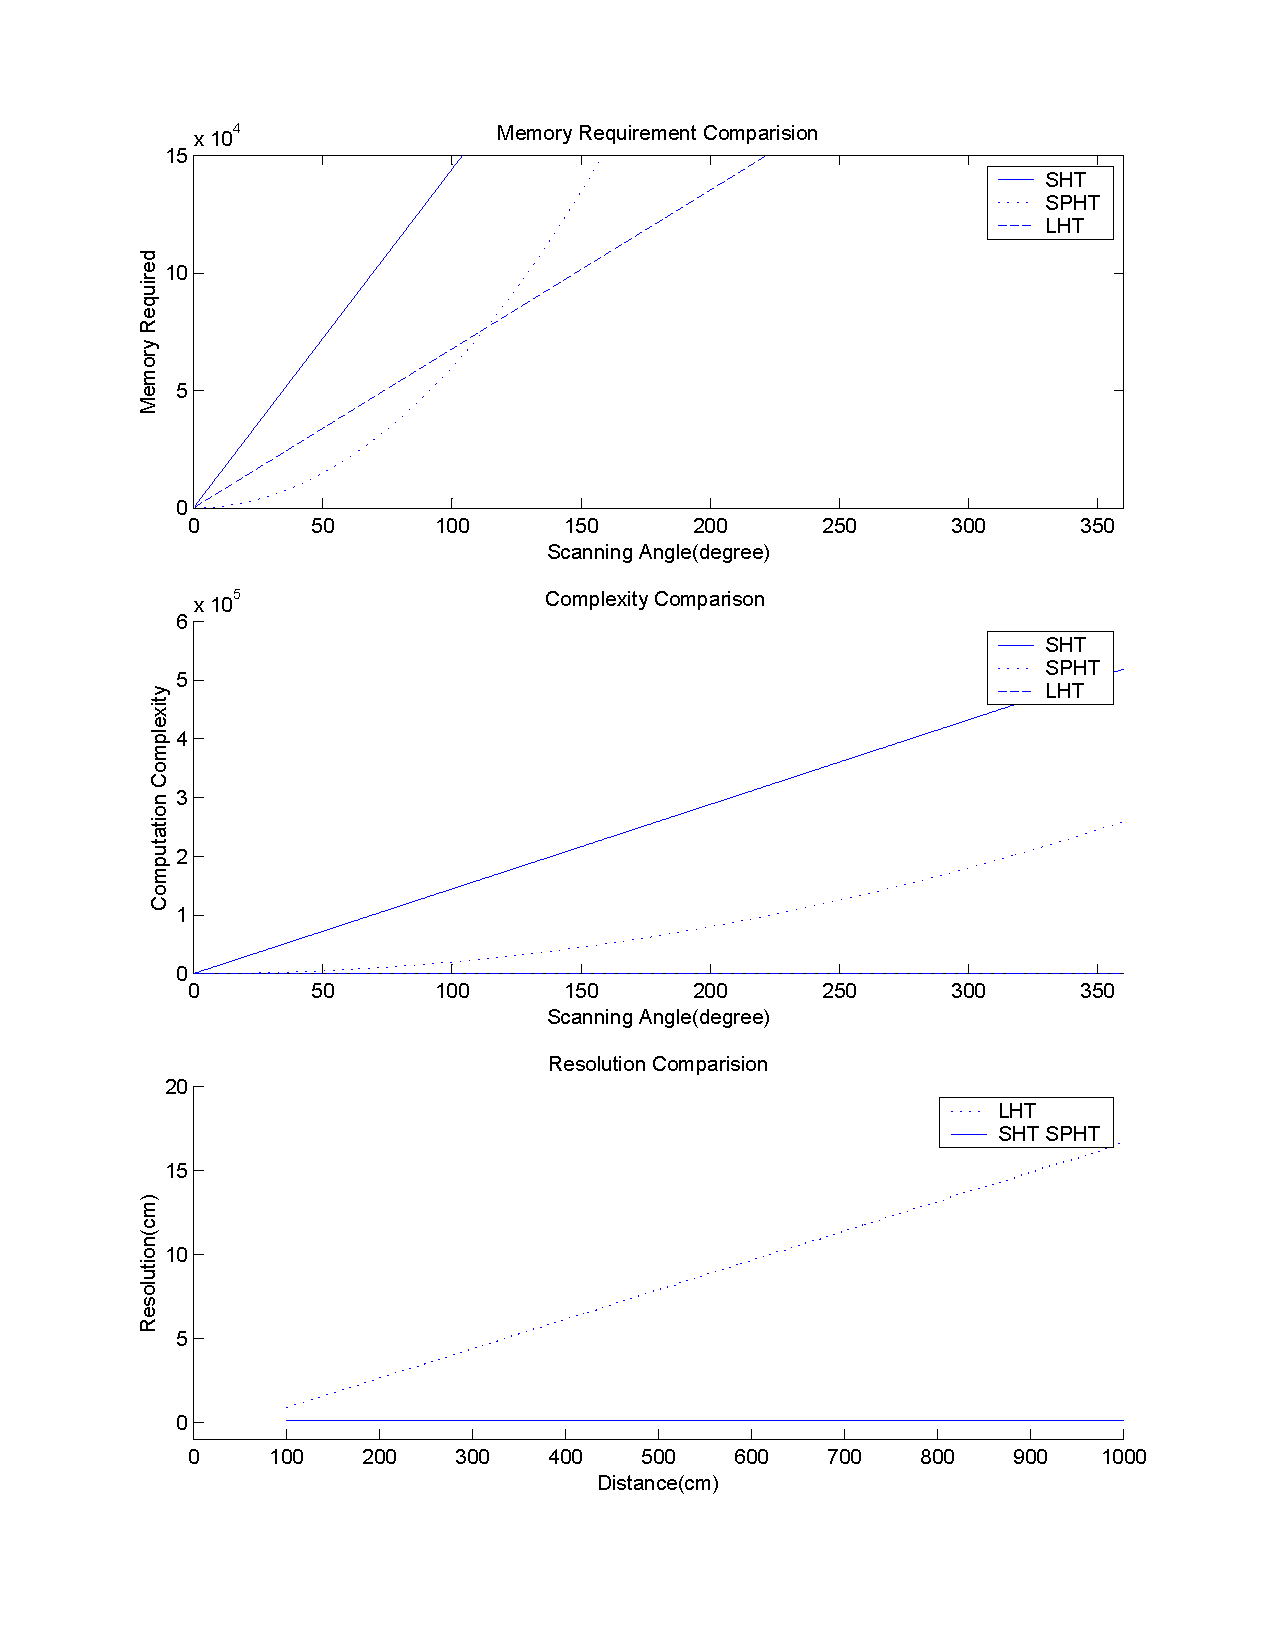
\includegraphics[width=0.45\textwidth,height=0.48\textwidth]{img/SPHTLHT}
    \caption{The Comparison of Sparse, Log and Standard Hough Transform} \label{fig:SPHTLHT}
\end{figure}
%%%%%%%%%%%%%%%%%%pole fit
\subsection{Task-Dependent Segmentation}
\label{sec24}


To process 2D laser data, segmentation is more complicated than in the case of 1D laser data. The idea of task-dependent segmentation is to simplify the situation by making a better use of the known information. Currently, we use lamp pole and side walk as landmarks to calibrate the odometry system of the mobile robot.

Lamp pole is an important landmark in a parking lot. Figure~\ref{fig:polefit} is the simulated data of a lamp pole from a 2D laser scanner mounted on T4, the mother robot  vehicle for ODIS. Here we assume that the lamp pole is perpendicular to the ground and the ground is flat. The task is to segment the raw data so that the position of the center of the lamp pole (cylinder) can be computed by some fitting algorithms. Figure~\ref{fig:polefitimg} is the image of the lamp pole that is projected to the ground. Here, our actual task is  to separate the ground from the lamp pole. Figure~\ref{fig:polefitedge} is the edge detection result of Fig.~\ref{fig:polefitimg}. Figure~\ref{fig:polefitElm} is the 3D object when we project the edge in Fig.~\ref{fig:polefitedge} back to the 3D space. At last, we set a threshold to eliminate those points too close to each other. The result is shown in Fig.~\ref{fig:polefitElm}. 

After projecting these points to the ground, we can get a circle with the same center of the 3D lamp pole. In other words, when we feed the result of the segmentation to our fitting algorithms, we can get the position of the feature points. Then the relative position of the landmark will be available for mobile robot odometry calibration, or localization. 

Another important landmark is the convex corner of the side walk. Since the height of side walk in a specific parking lot is constant, we can set a threshold to segment the ground and the upper layer. The segmentation is straightforward and  we will not discuss it here due to space limitation. 

\begin{figure}
\begin{minipage}[t]{0.23\textwidth}
    \centering
    \includegraphics[angle=90,width=\textwidth]{img/sparsehough}
    \caption{An Example of Sparse Hough Transform} \label{fig:spht}
\end{minipage}
\begin{minipage}[t]{0.23\textwidth}
    \centering
    \centering\includegraphics[width=\textwidth]{img/PoleFit}
     \caption{Lamp Pole Simulation Data} \label{fig:polefit}
\end{minipage}
\end{figure}

\begin{figure}[!htb]
    \begin{minipage}[t]{0.23\textwidth}
       \centering\includegraphics[width=\textwidth]{img/PoleFitImg}
       \caption{Projected Lamp Pole Image} \label{fig:polefitimg} 
    \end{minipage} %
    \begin{minipage}[t]{0.23\textwidth}
        \centering\includegraphics[width=\textwidth]{img/PoleFitEdge}
        \caption{The Edge Detection on Lamp Pole Image} \label{fig:polefitedge}
    \end{minipage}
\end{figure}

\begin{figure}[!htb]
    \begin{minipage}[t]{0.23\textwidth}
        \centering\includegraphics[width=\textwidth]{img/PoleFitAfterEdgeDet}
        \caption{Reverse The Edge of Lamp Pole Image} \label{fig:polefitafteredgedet}
    \end{minipage} %
    \begin{minipage}[t]{0.23\textwidth}
        \center\includegraphics[width=\textwidth]{img/PoleFitEliminateStacks} 
        \caption{Lamp Pole Data After Segmentation} \label{fig:polefitElm}
    \end{minipage}
\end{figure}






%***************************************************
\section{Template Fitting Algorithms}
\label{sec3}

With  properly segmented data sets from a laser scan,  it is not certain which   template in the template library is to be used for the object fitting, without human involvement. A viable way is to try all templates in the library and then pick the ``best'' one via an arbitrator based on some rules from the possible prior knowledge about the objects in the static and uncertain environment.

For computational efficiency, we focus ourself on the algebraic fitting which does not require any iteration. For geometrical fitting, is may make more sense but the iterations may take a long time and some times, convergence cannot be guaranteed. It is of course, when possible, beneficial to use the geometrical fitting result to cross-validate that from the algebraic fitting.

Most of our codes for fitting are tested in Matlab and then converted to C++ \footnote{We used Dr. Robert Davies' free C++ library ``\texttt{NewMat}'' downloadable from \texttt{http://webnz.com/robert/cpp\_lib.htm}.} which are ready for running in our Linux box.




\subsection{Algebraic Circle Fit}
\label{sec31}

When the radius of a circle is unknown,   a simple algebraic circle fitting method can be applied to find the best fit circle in the   least  squares (LS) sense. 

Given a set of points with coordination $\{ (x_i,y_i), i=1,2, \cdots, n\} $,   find the best parameters $a_1, \cdots, a_4$ in the circle equation
$$a_1 (x^2+y^2) + a_2 x + a_3 y +a_4=0,$$
such that
the algebraic error 
%$\varepsilon = \sum_{i=1}^{n} (\sqrt{ (x_i-x_c)^2+(y_i-y_c)^2 } - r_c^2)$ 
is to be  minimized. The center of the circle is $(x_c, y_c)$ with $x_c = -\frac{a_2}{2 a_1}, $ $y_c = -\frac{a_3}{2 a_1}. $

Let ${\mathbf a}= [a_{1},   a_{2},  a_{3},  a_{4}]^T$. Construct  the matrix $ \mathbf{D}$ as
\[
 \mathbf{D}=\begin{bmatrix}
  x_1^2+y_1^2 & x_1 & y_1 & 1 \\
  x_2^2+y_2^2 & x_2 & y_2 & 1 \\
  x_3^2+y_3^2 & x_3 & y_3 & 1 \\
  \vdots & \vdots& \vdots & \vdots \\
  x_n^2+y_n^2 & x_n & y_n & 1 \\
\end{bmatrix}.\]
Then, the LS   solution of equation $$\mathbf{D a}=0$$ is simply given by the 
 SVD (singular value decomposition).  
via \texttt{[U,V,D]=SVD()}. Denote $\mathbf{V}=[v_1, v_2,\cdots,v_n].$ Then, the solution is simply $\mathbf{a}=v_4$.
Figure~\ref{fig:CirFit} shows a typical circle fit to an experimental 1D laser scan data set.

\begin{figure}
    \centering
    \includegraphics[width=0.3\textwidth]{img/CircleFit} \caption{Circle Fit} \label{fig:CirFit}
\end{figure}



\subsection{Circle Fit with a Known Radius}
\label{sec32}


Some of the round objects in the static uncertain environment may have known radii.
So, although simpler, it is practically desirable to perform the circle fit with a known radius. Here we use the geometrical error for the fitness performance index.

%This approach based on algebraic circle fit in order to achieve a better precision. 

Given a set of points with coordinates $\{ (x_i,y_i), i=1,2, \cdots, n\} $,   find the best parameters $x_c$ and $y_c$, the center coordinate of the circle
\[
(x-x_c)^2+(y-y_c)^2  - R^2=0
\]
where $R$ is the known radius, such that the geometric error 
 $\varepsilon = \sum_{i=1}^{n} (\sqrt{ (x_i-x_c)^2+(y_i-y_c)^2 } - R)^2$ 
is minimized.  

Via the gradient of $\varepsilon$ with respect to $x_c$ and $y_c$, an iterative scheme for  $x_c$ and $y_c$ can be formulated and implemented. Since $R$ is known, the convergence process is quite reliable and fast.
%
%$$J=\left[ \matrix{
%\frac{\partial Error}{\partial x_i} & \frac{\partial Error}{\partial y_i} } \right] $$
%$$= \left[ \matrix{
%\frac{(x_i-x_c)}{\sqrt{(x_i-x_c)^2+(y_i-y_c)^2}} & \frac{(y_i-y_c)}{\sqrt{(x_i-x_c)^2+(y_i-y_c)^2}}
%} \right] $$
%Then we can use gradient converge approach to update the origin by
%$$ J h + Error = 0 $$
%$$ \left[ \matrix{x_c & y_c} \right] = \left[ \matrix{x_c & y_c} \right] + h $$




\subsection{Ellipse Fit}
\label{sec33}

We skip this part due to the space limit. The ellipse fitting codes are included in the {\tt zip} file downloadable from the URL given in the first page of this paper. More technique details are available upon request.
%The general form of an ellipse is described by
%\[
%a_1 x^2 + a_2 x y + a_3 y^2 + a_4 x + a_5 y + a_6 =0.
%\]
%The ellipse fit problem is very similar to the algebraic circle fit method presented in 
%Sec.~\ref{sec31}. 
%
%%Given two vector $(\mathbf{x}, \mathbf{y})$ with the same size, solve the equation $ M\mathbf{a} = 0$ by means of least mean square, where 
%Here the matrix sent for SVD is given by
%$$  \mathbf{D}= \begin{bmatrix}
%x_1^2 & x_1 y_1 & y_1^2 & x_1 & y_1 & 1 \\
%x_2^2 & x_2 y_2 & y_2^2 & x_2 & y_2 & 1 \\
%x_3^2 & x_3 y_3 & y_3^2 & x_3 & y_3 & 1 \\
%\vdots & \vdots & \vdots& \vdots& \vdots& \vdots \\
%x_n^2 & x_n y_n & y_n^2 & x_n & y_n & 1 \\
%\end{bmatrix} $$
% and ${\mathbf a}= [a_{1},  \cdots,  a_{6}]'$
%%
%Same as circle fit, we can do SVD decomposition for matrix $M$, $[U, S, V]= SVD(M)$, and $V=\left[\matrix{%
%v_1 & v_2 & v_3 & \cdots } \right] $. The solution is $v_6$. 


 

\subsection{Plane Fit}
\label{sec3_planefit}



Different from the above fitting method mainly for 1D laser scan data set, the methods of this subsection and the next subsection are designed for 2D laser scanner data processing. Actually, the acquired data from a 2D laser scanner is a 3D  array, as mentioned in Sec.~\ref{sec2}.
The goal of the plane fitting problem is to find the optimal coefficients $a_1, a_2, a_3, a_4$, such that
$$  \begin{bmatrix}
    x_1 & y_1 & z_1 & 1 \\
    x_2 & y_2 & z_2 & 1 \\
    x_3 & y_3 & z_3 & 1 \\
    \vdots&\vdots&\vdots&\vdots \\
    x_n & y_n & z_n & 1  \\
    \end{bmatrix}
    \begin{bmatrix}
    a_1 \\ a_2\\ a_3\\ a_4 \\
    \end{bmatrix} =0 $$
has a solution in LS sense. Again, we can use the SVD technique for the plane fitting.






\subsection{3D Corner Fit/Detection}
\label{sec3_3dcornerfit}

Corner in the context of 2D image processing is one of the basic image features and has been extensively studied in~\cite{Ruzon99Corner,Smith97Susan}. For 3D corner detection, we can project the 3D corner to a 2D surface and detect the corner in 2D. This method, although simple, may not be able to detect some corners in certain 3D configurations. Here, we propose two effective 3D corner fit algorithms. 

The first method fits an intersection point of 3 planes as the corner. So there is no limitation on whether the corner is convex or concave. The disadvantage of this algorithm  is that it can not fit corner without a prior step for plane segmentation. 

This corner fit problem is to find the best corner $\{x^*,y^*,z^*\}$, such that
$$\begin{bmatrix}
    A_1 & B_1 & C_1 \\
    A_2 & B_2 & C_2 \\
    A_3 & B_3 & C_3 \\
    \vdots & \vdots& \vdots \\
    A_n & B_n & C_n \\
    \end{bmatrix}
    \begin{bmatrix}
    x^* \\ y^* \\ z^* \\ 
    \end{bmatrix}
+
    \begin{bmatrix}
    D_1 \\ D_2 \\ D_3 \\ \vdots \\ D_n \\
    \end{bmatrix}
=
    \begin{bmatrix}
    e_1 \\ e_2 \\ e_3 \\ \vdots \\ e_n \\
    \end{bmatrix}
$$
or $M P = -D$, where $\begin{bmatrix} x^* & y^* & z^*  \end{bmatrix} = P^T$,  $\sqrt{\sum_i  e_i^2}$ is minimized. Based on the projection theorem, the solution is simply $P =(M^T M)^{-1} M^T (-D)$


The second algorithm can fit corners directly from the 3D point set. This approach eliminates the requirement on segmentation. We can separate points to small subsets, and then fit them by the following corner fit function. The limitation of the algorithm is that the corner function is only suitable for convex and symmetric corners. The proposed corner function is
described by
\[
z=e^{k_1(x-x_0)^2+k_2(y-y_0)^2+k_3}
\]
where $k_1, k_2, k_3, x_0, y_0$ are parameters to be fit. In LS sense, we can re-formulate the above fitting problem into 
    $$\begin{bmatrix}
    x_1^2 & x_1 & y_1^2 & y_1 & 1 \\
    x_2^2 & x_2 & y_2^2 & y_2 & 1 \\
    \vdots& \vdots&\vdots&\vdots&\vdots \\
    x_n^2 & x_n & y_n^2 & y_n & 1 \\
    \end{bmatrix}
    \begin{bmatrix}
    c_1 \\ c_2 \\ c_3 \\ c_4 \\ c_5 \\ 
    \end{bmatrix}
    =
    \begin{bmatrix}
    \log(z_1) \\ \log(z_2) \\ \vdots \\ \log(z_n) \\
    \end{bmatrix}.     $$
The rest of the algorithm is the same as in the previous 3D corner fitting method.

%the $\left[\matrix{c_1 & c_2 & c_3 & c_4 & c_5} \right]$ with minimum norm is the solution we want. This question can be solved by the same approach of the corner fit. 


\section{Arbitrator}
If the identity of the object is not clearly known, arbitration is necessary to find the suitable template for the fitting algorithm. The basic idea is that we can try to fit the unknown shape to all suspected models, and then find the best fit with respect to the geometry error. 

Since we used algebraic fitting, the geometrical error have to be re-calculated. Here, we use the circle fit as an example.

For a circle $a_1 (x^2+y^2) + a_2 x + a_3 y +a_4=0$, the geometry error $E$ is 
$$E=\sum_{i=1}^{n}\left|\sqrt{(x_i+\frac{a_2}{2 a_1})^2+(y_i+\frac{a_3}{2 a_1})^2-R}\right|,$$ where $R=\sqrt{{a_2^2 \over {4 a_1^2}}+{a_3^2 \over {4 a_1^2}}-{a_4 \over a_1}}.$

%
%A general form for an ellipse is $a_1 x^2 + a_2 x y + a_3 y^2 + a_4 x + a_5 y + a_6 =0$, or we can write it in the matrix and vector form $||L R (\mb{z}-\mb{z_0})||=1$, where 
%$L=
%\bbm
%  1/a & 0 \\
%  0 & 1/b
%\ebm$, 
%$R=
%\bbm
%  \cos(\theta) & \sin(\theta) \\
%  -\sin(\theta) & \cos(\theta)
%\ebm $
%, $\mb{z}=
%\bbm    x & y   \ebm ^T$ is a point on the ellipse, and $\mb{z_0}= \bbm x_0 & y_0 \ebm ^T $ is the center of the ellipse. $a$ and $b$ are the long and short axis of the ellipse. $\theta$ is the rotation angle from $x$ axis of the coordinate system to the long axis of the ellipse. We can prove 
%\begin{eqnarray*}
%a_1&=a^2\sin(\theta)^2+b^2\cos(\theta)^2 \\
%a_2&=2\sin(\theta)\cos(\theta)(b^2-a^2)\\
%a_3&=a^2\cos(\theta)^2+b^2\sin(\theta)^2
%\end{eqnarray*}
%,or $$\bbm a_1 \\ a_3 \ebm= 
%\bbm \sin(\theta)^2 & \cos(\theta)^2 \\
%    \cos(\theta)^2 & \sin(\theta)^2 \ebm
%\bbm a^2 \\ b^2 \ebm.
%$$
%So, $\tan(2\theta)=\frac{a_2}{a_3-a_1}$, and 
%$$
%\bbm a^2 \\ b^2 \ebm=
%\begin{cases}
%    \bbm \sin(\theta)^2 & \cos(\theta)^2 \\
%        \cos(\theta)^2 & \sin(\theta)^2 \ebm ^{-1} \bbm a_1 \\ a_3 \ebm 
%    & \text{If $\theta\neq\pi/4$}, \\
%    \bbm a_1-a_2/2 \\ a_1+a_2/2 \ebm 
%    & \text{If $\theta=\pi/4$}.
%\end{cases} 
%$$
%Since $a\geq 0$ and $b\geq 0$, we can get $L$ now. Define $\mb{z_r}=R(\mb{z}-\mb{z_r})$. The Lagrangian is 
%$$ L(\mb{z_r},\lambda)=(\mb{p}_i-\mb{z_r})^T(\mb{p}_i-\mb{z_r})+\lambda(L\mb{z}_r)^T(L\mb{z}_r), $$
%where $\mb{p}_i=\bbm x_i & y_i \ebm ^T$ is the $i^\text{th}$ point of the data set. This leads to the necessary condition $(I+\lambda L^T L)\mb{z}_r=\mb{p}_i.$ Decompose $L$ to $L=U\Sigma V^T$, and define $\mb{e}=V^T\mb{p}_i$. Then we have $L\mb{z}_r(\lambda)=U\Sigma (I+\lambda \Sigma^2)^{-1} \mb{e}$. According to $||L \mb{z}_r ||=1$, we have $f(\lambda)=\sum_{j=1}^n \frac{e_j^2\sigma_j^2}{(1+\lambda \sigma_j^2)^2} =1 $. Find the solution $\lambda_i^\ast$ for $\mb{p}_i$, i.e.,$f(\lambda_i^\ast)=1$, then the minimum distance between the point $\mb{p}_i$ and the ellipse $|| L R(\mb{z}-\mb{z}_0)||=1$ is $|| \mb{p}_i - L \mb{z}_r(\lambda_i^\ast)||$. For a cluster of points, the geometry error is 
%$$ E=\sum^n_{i=1} ||\mb{p}_i-\mb{z}_r(\lambda_i^\ast) || $$
%
%For a plane $a_1 x + a_2 y + a_3 z + a_4 =0,$
%and a point $\mb{p}_i(x_i,y_i,z_i)$, easy to prove the geometry error $E$ is 
%$$E=\sum_{i=1}^n\frac{|a_1 x_i+ a_2 y_i +a_3 z_i + a_4|}{\sqrt{a_1^2+a_2^2+a_3^2}} $$


The real objects, e.g., lamp pole and curb, are too complex for computers to identify directly. We follow the idea of ``{\em segmentation--fitting}'' to represent complex objects in basic geometry shapes, i.e., circle, ellipse, line, plane, corner. The geometry errors are the index of the ``likelihood'' for those fittings. The arbitrator can be regarded as a processor to reduce the raw data to simple, abstract and higher level information for the decision maker in the robot's higher-level control. Figure~\ref{fig:arb} is the flow chart of our arbitrator. Since our robot works in the structured unknown environment, we can put all possible templates in the object library, and add more if the environment is changed. This extendable feature is important in real intelligent robot systems. 
%real world applications.  %After got a set of 3D data, we will do segmentation, then fit them with different model in the library. According to different model, we can choose proper fitting algorithms, % which will give back the geometry errors for the fitting. 



%In the final version of this paper,   we will include the section on ``Arbitrator'' or ``Object Decision'' as well as the related experimental results. 

\begin{figure}
  \centering
  \includegraphics[width=0.35\textwidth]{img/Arbitrator}\\
  \caption{The Flow Chart of Arbitration and Object Decision}\label{fig:arb}
\end{figure}



%%%%%%%%%%%%%%%%%%%%%%%%%%%%%%%%%%%%%%%%%%%%%%%%%%%%%%%%%%%%%%%%%%%%%%%%%%%
\section{Concluding Remarks}  
\label{sec6}
%%%%%%%%%%%%%%%%%%%%%%%%%%%%%%%%%%%%%%%%%%%%%%%%%%%%%%%%%%%%%%%%%%%%%%%%%%% 
   
This paper presents some techniques for sensing and perception for an
omnidirectional ground autonomous vehicle equipped with a laser scanner. In an
assumed structured environment (static but uncertain), the sensing data processing methods for both 1D and 2D laser scanners are discussed. Raw data are segmented to lines, circles,
ellipses, planes and corners by task dependent segmentation algorithms.  Each
subset of data is then fit by a known template shape as listed above.  

Our immediate effort is to make use of these medium level information in our  vehicle to infer its relative position with respect to the known landmarks and in turn help to determine its absolute
position on the map, a procedure known as mobile robot localization.
Other future efforts include (1) the motion estimation of dynamic obstacle(s) by assuming that the environment is dynamic uncertain; (2) the fusion with sonar, laser scanner and image sensing information for local map building and
 (3)  relative navigation  without  absolution position information (or inertial/world coordinates) via sensor fusion and spatial filtering.





\section*{Acknowledgment}
The authors would like to acknowledge the fruitful discussions with 
CSOIS members in Vetronics Group and Intelligent Behavior Group. In particular, 
  the authors are grateful to Professor Kevin L. Moore,  Director of CSOIS, for his   support  of this work.
 
\bibliography{csois1,csois2,laser}
 
\end{document}
 

% cut paste this two bib entries in your "laser.bib"
